\documentclass[12pt]{article}

\usepackage{ee143report}
\usepackage{verbatim}
\usepackage{graphicx, float}
\usepackage{enumerate}
\usepackage{amsmath}
\usepackage{bookmark}
\usepackage{pdflscape}
\usepackage{multirow}
\usepackage{hyperref}

\DeclareMathOperator{\V}{V}
\DeclareMathOperator{\A}{A}
\DeclareMathOperator{\F}{F}
\DeclareMathOperator{\mA}{mA}
\DeclareMathOperator{\mW}{mW}
\DeclareMathOperator\bit{bit}
\DeclareMathOperator\byte{byte}
\DeclareMathOperator\word{word}

\author{Astrid Yu}
\title{Arduino Ohmmeter}
\expNum{6}
\titlegraphic{
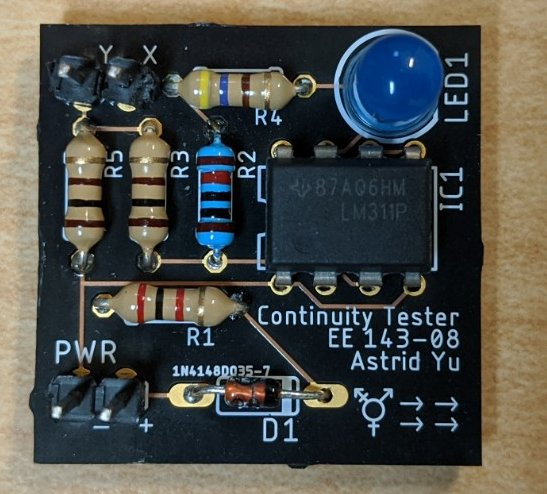
\includegraphics[width=0.6\linewidth]{img/top.jpg}
}

\begin{document}
\maketitle

\section*{Introduction}

In this experiment, the PCB designed in Lab 4 will be assembled. The device will be tested after assembly, and if necessary, its function will be troubleshooted. 

\section*{Analysis}

The PCB was received back from OSHPark and assembled.

\begin{figure}[H]
  \centering
  \includegraphics[width=0.85\linewidth]{img/emp.jpg}
  \caption{Received PCBs.}
  \label{}
\end{figure}
        
\begin{figure}[H]
  \centering
  \includegraphics[width=0.4\linewidth]{preview-top.png}
  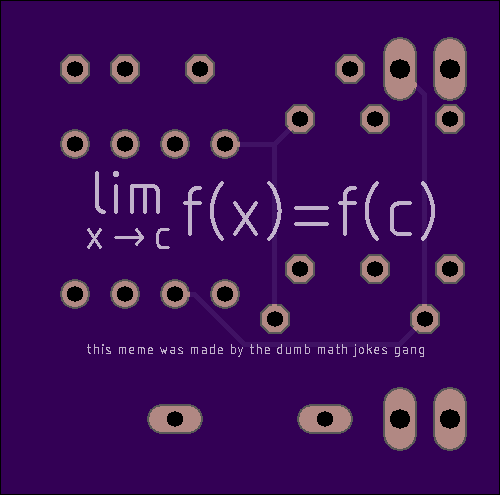
\includegraphics[width=0.4\linewidth]{preview-bottom.png}
  \caption{The previews that OSHPark generated.}
  \label{fig:preview}
\end{figure}


\subsection*{Section 2 -- Electrical Test}

The circuit's functionality was confirmed.

\begin{figure}[H]
  \centering
  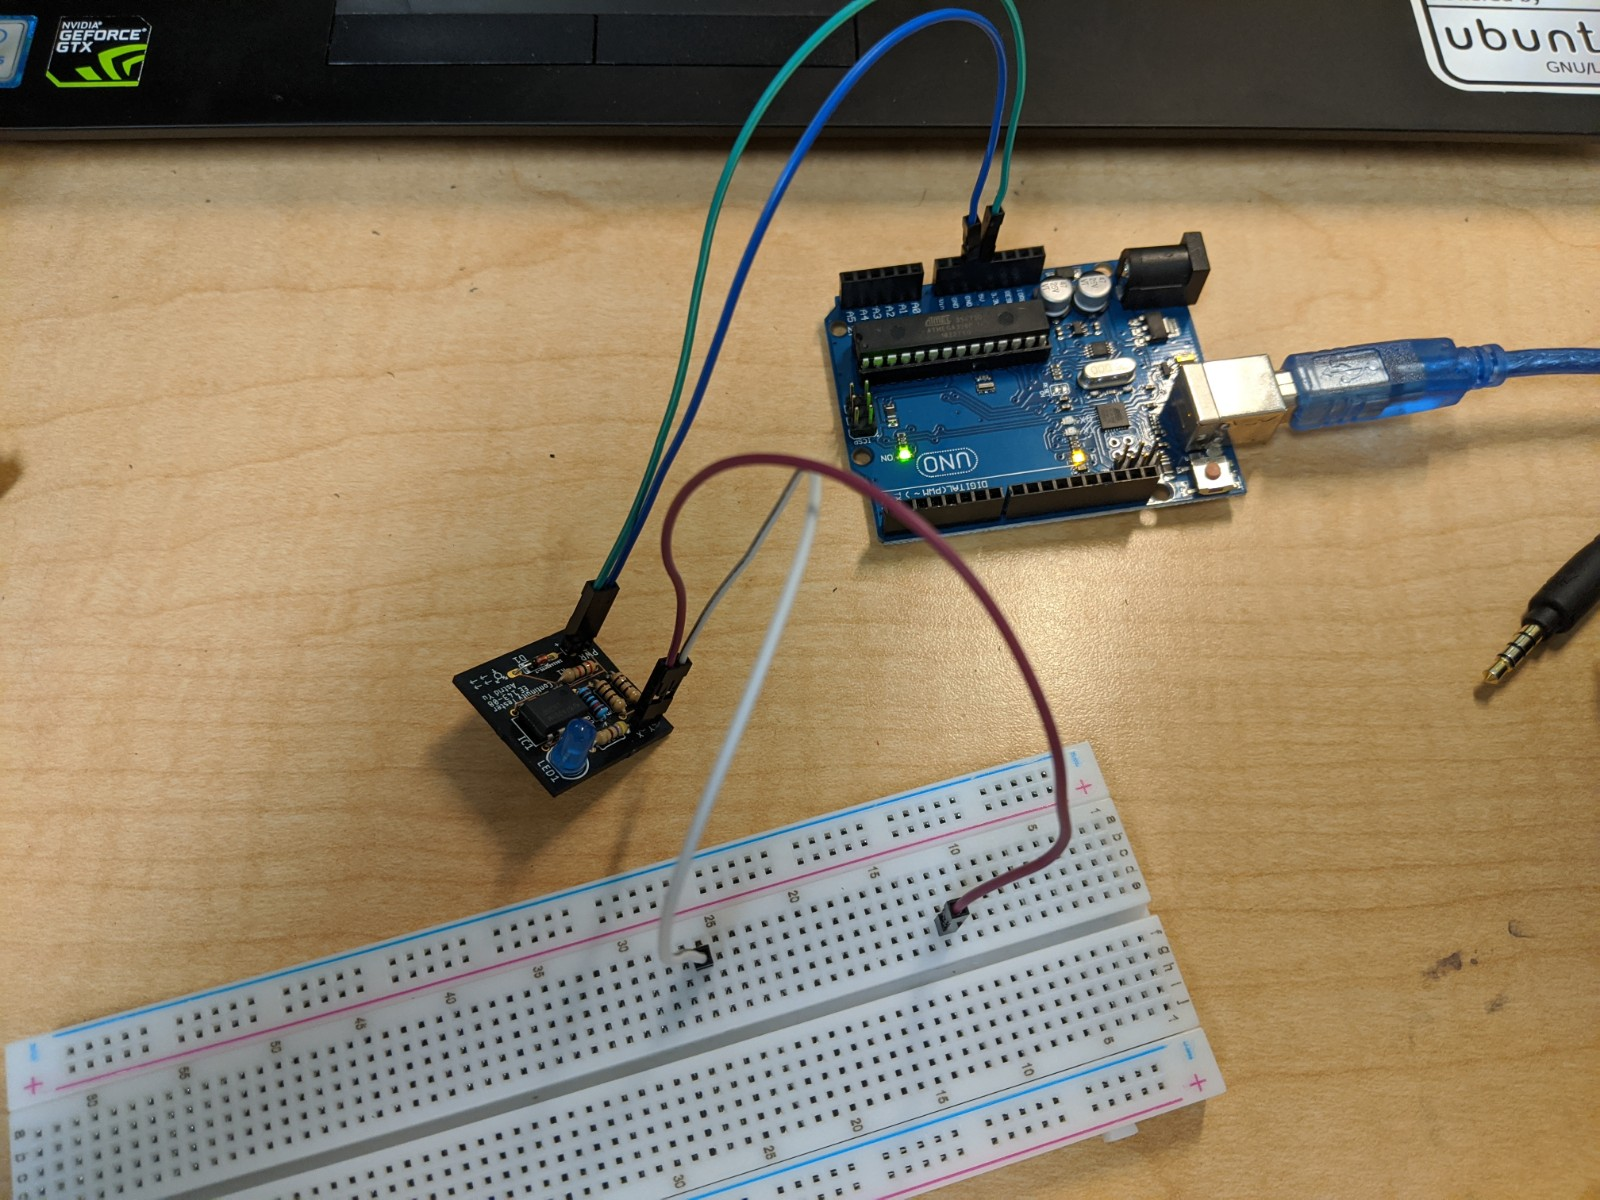
\includegraphics[width=0.8\linewidth]{img/open.jpg}
  \caption{The LED is off when there is an open.}
  \label{}
\end{figure}

\begin{figure}[H]
  \centering
  \includegraphics[width=0.8\linewidth]{img/short.jpg}
  \caption{The LED is on when there is a short.}
  \label{}
\end{figure}

\subsection*{Section 3 -- Troubleshooting}

Because the circuit was confirmed to work, no troubleshooting was necessary. 

\section*{Discussion Questions}

\subsection*{Section 2}

\begin{figure}[H]
  \centering
  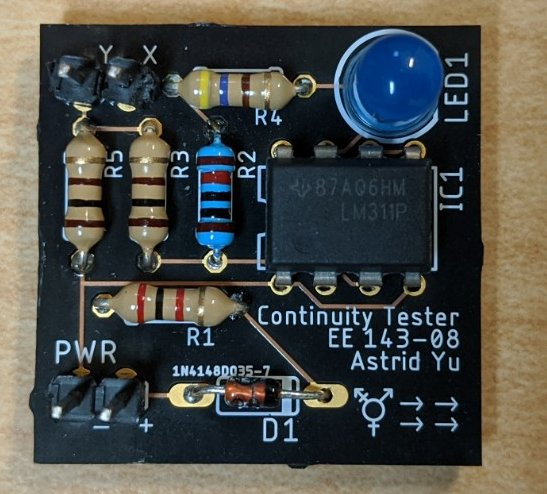
\includegraphics[width=0.45\linewidth]{img/top.jpg}
  \includegraphics[width=0.45\linewidth]{img/bot.jpg}
  \caption{The top and bottom of the soldered board.}
  \label{}
\end{figure}

\subsection*{Section 3}

N/A -- No troubleshooting was necessary.

\section*{Conclusion}

The circuit was successfully assembled by soldering. It was confirmed to work through functional testing. Troubleshooting was not necessary because the circuit functioned flawlessly. 

\end{document}
